\documentclass[twoside]{book}

% Packages required by doxygen
\usepackage{fixltx2e}
\usepackage{calc}
\usepackage{doxygen}
\usepackage[export]{adjustbox} % also loads graphicx
\usepackage{graphicx}
\usepackage[utf8]{inputenc}
\usepackage{makeidx}
\usepackage{multicol}
\usepackage{multirow}
\PassOptionsToPackage{warn}{textcomp}
\usepackage{textcomp}
\usepackage[nointegrals]{wasysym}
\usepackage[table]{xcolor}

% Font selection
\usepackage[T1]{fontenc}
\usepackage[scaled=.90]{helvet}
\usepackage{courier}
\usepackage{amssymb}
\usepackage{sectsty}
\renewcommand{\familydefault}{\sfdefault}
\allsectionsfont{%
  \fontseries{bc}\selectfont%
  \color{darkgray}%
}
\renewcommand{\DoxyLabelFont}{%
  \fontseries{bc}\selectfont%
  \color{darkgray}%
}
\newcommand{\+}{\discretionary{\mbox{\scriptsize$\hookleftarrow$}}{}{}}

% Page & text layout
\usepackage{geometry}
\geometry{%
  a4paper,%
  top=2.5cm,%
  bottom=2.5cm,%
  left=2.5cm,%
  right=2.5cm%
}
\tolerance=750
\hfuzz=15pt
\hbadness=750
\setlength{\emergencystretch}{15pt}
\setlength{\parindent}{0cm}
\setlength{\parskip}{3ex plus 2ex minus 2ex}
\makeatletter
\renewcommand{\paragraph}{%
  \@startsection{paragraph}{4}{0ex}{-1.0ex}{1.0ex}{%
    \normalfont\normalsize\bfseries\SS@parafont%
  }%
}
\renewcommand{\subparagraph}{%
  \@startsection{subparagraph}{5}{0ex}{-1.0ex}{1.0ex}{%
    \normalfont\normalsize\bfseries\SS@subparafont%
  }%
}
\makeatother

% Headers & footers
\usepackage{fancyhdr}
\pagestyle{fancyplain}
\fancyhead[LE]{\fancyplain{}{\bfseries\thepage}}
\fancyhead[CE]{\fancyplain{}{}}
\fancyhead[RE]{\fancyplain{}{\bfseries\leftmark}}
\fancyhead[LO]{\fancyplain{}{\bfseries\rightmark}}
\fancyhead[CO]{\fancyplain{}{}}
\fancyhead[RO]{\fancyplain{}{\bfseries\thepage}}
\fancyfoot[LE]{\fancyplain{}{}}
\fancyfoot[CE]{\fancyplain{}{}}
\fancyfoot[RE]{\fancyplain{}{\bfseries\scriptsize Generated by Doxygen }}
\fancyfoot[LO]{\fancyplain{}{\bfseries\scriptsize Generated by Doxygen }}
\fancyfoot[CO]{\fancyplain{}{}}
\fancyfoot[RO]{\fancyplain{}{}}
\renewcommand{\footrulewidth}{0.4pt}
\renewcommand{\chaptermark}[1]{%
  \markboth{#1}{}%
}
\renewcommand{\sectionmark}[1]{%
  \markright{\thesection\ #1}%
}

% Indices & bibliography
\usepackage{natbib}
\usepackage[titles]{tocloft}
\setcounter{tocdepth}{3}
\setcounter{secnumdepth}{5}
\makeindex

% Hyperlinks (required, but should be loaded last)
\usepackage{ifpdf}
\ifpdf
  \usepackage[pdftex,pagebackref=true]{hyperref}
\else
  \usepackage[ps2pdf,pagebackref=true]{hyperref}
\fi
\hypersetup{%
  colorlinks=true,%
  linkcolor=blue,%
  citecolor=blue,%
  unicode%
}

% Custom commands
\newcommand{\clearemptydoublepage}{%
  \newpage{\pagestyle{empty}\cleardoublepage}%
}

\usepackage{caption}
\captionsetup{labelsep=space,justification=centering,font={bf},singlelinecheck=off,skip=4pt,position=top}

%===== C O N T E N T S =====

\begin{document}

% Titlepage & ToC
\hypersetup{pageanchor=false,
             bookmarksnumbered=true,
             pdfencoding=unicode
            }
\pagenumbering{alph}
\begin{titlepage}
\vspace*{7cm}
\begin{center}%
{\Large Cam and Eggs \\[1ex]\large 1.\+0 }\\
\vspace*{1cm}
{\large Generated by Doxygen 1.8.13}\\
\end{center}
\end{titlepage}
\clearemptydoublepage
\pagenumbering{roman}
\tableofcontents
\clearemptydoublepage
\pagenumbering{arabic}
\hypersetup{pageanchor=true}

%--- Begin generated contents ---
\chapter{Hierarchical Index}
\section{Class Hierarchy}
This inheritance list is sorted roughly, but not completely, alphabetically\+:\begin{DoxyCompactList}
\item \contentsline{section}{net.\+mobiledevelopment.\+camandeggs.\+Chicken}{\pageref{classnet_1_1mobiledevelopment_1_1camandeggs_1_1_chicken}}{}
\item \contentsline{section}{net.\+mobiledevelopment.\+camandeggs.\+Message}{\pageref{classnet_1_1mobiledevelopment_1_1camandeggs_1_1_message}}{}
\item \contentsline{section}{net.\+mobiledevelopment.\+camandeggs.\+Server}{\pageref{classnet_1_1mobiledevelopment_1_1camandeggs_1_1_server}}{}
\item App\+Compat\+Activity\begin{DoxyCompactList}
<<<<<<< .merge_file_RdUIYV
=======
\item \contentsline{section}{net.\+mobiledevelopment.\+camandeggs.\+Chicken\+Bio\+Activity}{\pageref{classnet_1_1mobiledevelopment_1_1camandeggs_1_1_chicken_bio_activity}}{}
>>>>>>> .merge_file_0ZKZVS
\item \contentsline{section}{net.\+mobiledevelopment.\+camandeggs.\+Main\+Activity}{\pageref{classnet_1_1mobiledevelopment_1_1camandeggs_1_1_main_activity}}{}
\begin{DoxyCompactList}
\item \contentsline{section}{net.\+mobiledevelopment.\+camandeggs.\+Add\+Eggs\+Activity}{\pageref{classnet_1_1mobiledevelopment_1_1camandeggs_1_1_add_eggs_activity}}{}
\end{DoxyCompactList}
\end{DoxyCompactList}
\item S\+Q\+Lite\+Open\+Helper\begin{DoxyCompactList}
\item \contentsline{section}{net.\+mobiledevelopment.\+camandeggs.\+Cam\+And\+Eggs\+S\+Q\+Lite\+Helper}{\pageref{classnet_1_1mobiledevelopment_1_1camandeggs_1_1_cam_and_eggs_s_q_lite_helper}}{}
\end{DoxyCompactList}
\end{DoxyCompactList}

\chapter{Class Index}
\section{Class List}
Here are the classes, structs, unions and interfaces with brief descriptions\+:\begin{DoxyCompactList}
\item\contentsline{section}{\hyperlink{classnet_1_1mobiledevelopment_1_1camandeggs_1_1_add_eggs_activity}{net.\+mobiledevelopment.\+camandeggs.\+Add\+Eggs\+Activity} }{\pageref{classnet_1_1mobiledevelopment_1_1camandeggs_1_1_add_eggs_activity}}{}
\item\contentsline{section}{\hyperlink{classnet_1_1mobiledevelopment_1_1camandeggs_1_1_cam_and_eggs_s_q_lite_helper}{net.\+mobiledevelopment.\+camandeggs.\+Cam\+And\+Eggs\+S\+Q\+Lite\+Helper} }{\pageref{classnet_1_1mobiledevelopment_1_1camandeggs_1_1_cam_and_eggs_s_q_lite_helper}}{}
\item\contentsline{section}{\hyperlink{classnet_1_1mobiledevelopment_1_1camandeggs_1_1_chicken}{net.\+mobiledevelopment.\+camandeggs.\+Chicken} }{\pageref{classnet_1_1mobiledevelopment_1_1camandeggs_1_1_chicken}}{}
<<<<<<< .merge_file_FaFMb8
=======
\item\contentsline{section}{\hyperlink{classnet_1_1mobiledevelopment_1_1camandeggs_1_1_chicken_bio_activity}{net.\+mobiledevelopment.\+camandeggs.\+Chicken\+Bio\+Activity} }{\pageref{classnet_1_1mobiledevelopment_1_1camandeggs_1_1_chicken_bio_activity}}{}
>>>>>>> .merge_file_ASjQkq
\item\contentsline{section}{\hyperlink{classnet_1_1mobiledevelopment_1_1camandeggs_1_1_main_activity}{net.\+mobiledevelopment.\+camandeggs.\+Main\+Activity} }{\pageref{classnet_1_1mobiledevelopment_1_1camandeggs_1_1_main_activity}}{}
\item\contentsline{section}{\hyperlink{classnet_1_1mobiledevelopment_1_1camandeggs_1_1_message}{net.\+mobiledevelopment.\+camandeggs.\+Message} }{\pageref{classnet_1_1mobiledevelopment_1_1camandeggs_1_1_message}}{}
\item\contentsline{section}{\hyperlink{classnet_1_1mobiledevelopment_1_1camandeggs_1_1_server}{net.\+mobiledevelopment.\+camandeggs.\+Server} }{\pageref{classnet_1_1mobiledevelopment_1_1camandeggs_1_1_server}}{}
\end{DoxyCompactList}

\chapter{Class Documentation}
\hypertarget{classnet_1_1mobiledevelopment_1_1camandeggs_1_1_add_eggs_activity}{}\section{net.\+mobiledevelopment.\+camandeggs.\+Add\+Eggs\+Activity Class Reference}
\label{classnet_1_1mobiledevelopment_1_1camandeggs_1_1_add_eggs_activity}\index{net.\+mobiledevelopment.\+camandeggs.\+Add\+Eggs\+Activity@{net.\+mobiledevelopment.\+camandeggs.\+Add\+Eggs\+Activity}}
Inheritance diagram for net.\+mobiledevelopment.\+camandeggs.\+Add\+Eggs\+Activity\+:\begin{figure}[H]
\begin{center}
\leavevmode
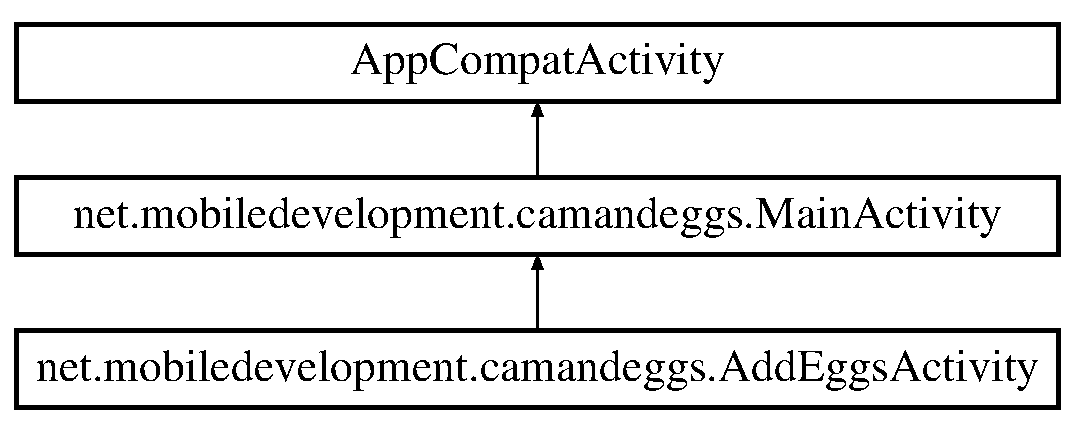
\includegraphics[height=3.000000cm]{classnet_1_1mobiledevelopment_1_1camandeggs_1_1_add_eggs_activity}
\end{center}
\end{figure}
\subsection*{Public Member Functions}
\begin{DoxyCompactItemize}
\item 
\mbox{\Hypertarget{classnet_1_1mobiledevelopment_1_1camandeggs_1_1_add_eggs_activity_a37b55b93ec8017a493248137bdd463c6}\label{classnet_1_1mobiledevelopment_1_1camandeggs_1_1_add_eggs_activity_a37b55b93ec8017a493248137bdd463c6}} 
void {\bfseries update\+Egg\+Total} (\hyperlink{classnet_1_1mobiledevelopment_1_1camandeggs_1_1_chicken}{Chicken} agnes, \hyperlink{classnet_1_1mobiledevelopment_1_1camandeggs_1_1_chicken}{Chicken} irma, \hyperlink{classnet_1_1mobiledevelopment_1_1camandeggs_1_1_chicken}{Chicken} petunia)
\item 
\mbox{\Hypertarget{classnet_1_1mobiledevelopment_1_1camandeggs_1_1_add_eggs_activity_a62dac758d87fac73409199fcaee39b93}\label{classnet_1_1mobiledevelopment_1_1camandeggs_1_1_add_eggs_activity_a62dac758d87fac73409199fcaee39b93}} 
void {\bfseries clear\+Database} (\hyperlink{classnet_1_1mobiledevelopment_1_1camandeggs_1_1_cam_and_eggs_s_q_lite_helper}{Cam\+And\+Eggs\+S\+Q\+Lite\+Helper} db, \hyperlink{classnet_1_1mobiledevelopment_1_1camandeggs_1_1_chicken}{Chicken} name)
\end{DoxyCompactItemize}
\subsection*{Public Attributes}
\begin{DoxyCompactItemize}
\item 
\mbox{\Hypertarget{classnet_1_1mobiledevelopment_1_1camandeggs_1_1_add_eggs_activity_aada00f2e6f6daefca183af4237e5405b}\label{classnet_1_1mobiledevelopment_1_1camandeggs_1_1_add_eggs_activity_aada00f2e6f6daefca183af4237e5405b}} 
Text\+View {\bfseries egg\+Total\+Text\+View}
\item 
\mbox{\Hypertarget{classnet_1_1mobiledevelopment_1_1camandeggs_1_1_add_eggs_activity_aedd93454d85bb4014e0d6de514f43eae}\label{classnet_1_1mobiledevelopment_1_1camandeggs_1_1_add_eggs_activity_aedd93454d85bb4014e0d6de514f43eae}} 
int {\bfseries agnes\+Total} = 0
\item 
\mbox{\Hypertarget{classnet_1_1mobiledevelopment_1_1camandeggs_1_1_add_eggs_activity_a8475dbe28b3b01309db240a335d04092}\label{classnet_1_1mobiledevelopment_1_1camandeggs_1_1_add_eggs_activity_a8475dbe28b3b01309db240a335d04092}} 
int {\bfseries egg\+Total} = 0
\end{DoxyCompactItemize}
\subsection*{Protected Member Functions}
\begin{DoxyCompactItemize}
\item 
void \hyperlink{classnet_1_1mobiledevelopment_1_1camandeggs_1_1_add_eggs_activity_af3bf6afd97bd62306181e63ee36a7ad0}{on\+Create} (Bundle saved\+Instance\+State)
\end{DoxyCompactItemize}


\subsection{Member Function Documentation}
\mbox{\Hypertarget{classnet_1_1mobiledevelopment_1_1camandeggs_1_1_add_eggs_activity_af3bf6afd97bd62306181e63ee36a7ad0}\label{classnet_1_1mobiledevelopment_1_1camandeggs_1_1_add_eggs_activity_af3bf6afd97bd62306181e63ee36a7ad0}} 
\index{net\+::mobiledevelopment\+::camandeggs\+::\+Add\+Eggs\+Activity@{net\+::mobiledevelopment\+::camandeggs\+::\+Add\+Eggs\+Activity}!on\+Create@{on\+Create}}
\index{on\+Create@{on\+Create}!net\+::mobiledevelopment\+::camandeggs\+::\+Add\+Eggs\+Activity@{net\+::mobiledevelopment\+::camandeggs\+::\+Add\+Eggs\+Activity}}
\subsubsection{\texorpdfstring{on\+Create()}{onCreate()}}
{\footnotesize\ttfamily void net.\+mobiledevelopment.\+camandeggs.\+Add\+Eggs\+Activity.\+on\+Create (\begin{DoxyParamCaption}\item[{Bundle}]{saved\+Instance\+State }\end{DoxyParamCaption})\hspace{0.3cm}{\ttfamily [protected]}}

Agnes

Irma

The documentation for this class was generated from the following file\+:\begin{DoxyCompactItemize}
\item 
<<<<<<< .merge_file_5NR9aa
Google Drive/\+C\+C\+B\+C/\+C\+S\+I\+T166/\+Camand\+Eggs/app/src/main/java/net/mobiledevelopment/camandeggs/Add\+Eggs\+Activity.\+java\end{DoxyCompactItemize}
=======
app/src/main/java/net/mobiledevelopment/camandeggs/Add\+Eggs\+Activity.\+java\end{DoxyCompactItemize}
>>>>>>> .merge_file_GYQj1S

\hypertarget{classnet_1_1mobiledevelopment_1_1camandeggs_1_1_cam_and_eggs_s_q_lite_helper}{}\section{net.\+mobiledevelopment.\+camandeggs.\+Cam\+And\+Eggs\+S\+Q\+Lite\+Helper Class Reference}
\label{classnet_1_1mobiledevelopment_1_1camandeggs_1_1_cam_and_eggs_s_q_lite_helper}\index{net.\+mobiledevelopment.\+camandeggs.\+Cam\+And\+Eggs\+S\+Q\+Lite\+Helper@{net.\+mobiledevelopment.\+camandeggs.\+Cam\+And\+Eggs\+S\+Q\+Lite\+Helper}}
Inheritance diagram for net.\+mobiledevelopment.\+camandeggs.\+Cam\+And\+Eggs\+S\+Q\+Lite\+Helper\+:\begin{figure}[H]
\begin{center}
\leavevmode
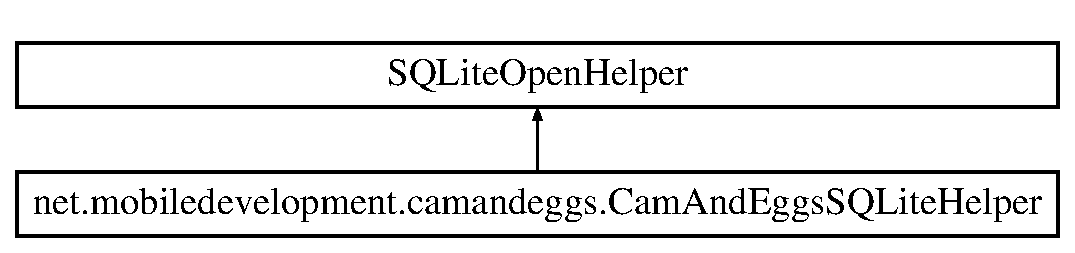
\includegraphics[height=2.000000cm]{classnet_1_1mobiledevelopment_1_1camandeggs_1_1_cam_and_eggs_s_q_lite_helper}
\end{center}
\end{figure}
\subsection*{Public Member Functions}
\begin{DoxyCompactItemize}
\item 
\mbox{\Hypertarget{classnet_1_1mobiledevelopment_1_1camandeggs_1_1_cam_and_eggs_s_q_lite_helper_a58cf8a1f9b82990dde258e7cf16c5008}\label{classnet_1_1mobiledevelopment_1_1camandeggs_1_1_cam_and_eggs_s_q_lite_helper_a58cf8a1f9b82990dde258e7cf16c5008}} 
{\bfseries Cam\+And\+Eggs\+S\+Q\+Lite\+Helper} (Context context)
\item 
\mbox{\Hypertarget{classnet_1_1mobiledevelopment_1_1camandeggs_1_1_cam_and_eggs_s_q_lite_helper_ac3c956b1798c178a75cca219182e74b5}\label{classnet_1_1mobiledevelopment_1_1camandeggs_1_1_cam_and_eggs_s_q_lite_helper_ac3c956b1798c178a75cca219182e74b5}} 
void {\bfseries on\+Create} (S\+Q\+Lite\+Database db)
\item 
\mbox{\Hypertarget{classnet_1_1mobiledevelopment_1_1camandeggs_1_1_cam_and_eggs_s_q_lite_helper_ac399432aaf515dea81cc90f8bd6ef568}\label{classnet_1_1mobiledevelopment_1_1camandeggs_1_1_cam_and_eggs_s_q_lite_helper_ac399432aaf515dea81cc90f8bd6ef568}} 
void {\bfseries on\+Upgrade} (S\+Q\+Lite\+Database db, int old\+Version, int new\+Version)
\item 
\mbox{\Hypertarget{classnet_1_1mobiledevelopment_1_1camandeggs_1_1_cam_and_eggs_s_q_lite_helper_a54d929d229814e9e915baaf25c726262}\label{classnet_1_1mobiledevelopment_1_1camandeggs_1_1_cam_and_eggs_s_q_lite_helper_a54d929d229814e9e915baaf25c726262}} 
void {\bfseries add\+Chicken} (\hyperlink{classnet_1_1mobiledevelopment_1_1camandeggs_1_1_chicken}{Chicken} chicken)
\item 
\mbox{\Hypertarget{classnet_1_1mobiledevelopment_1_1camandeggs_1_1_cam_and_eggs_s_q_lite_helper_aa7197a24b3e7d76842c1aa4d52c5a372}\label{classnet_1_1mobiledevelopment_1_1camandeggs_1_1_cam_and_eggs_s_q_lite_helper_aa7197a24b3e7d76842c1aa4d52c5a372}} 
\hyperlink{classnet_1_1mobiledevelopment_1_1camandeggs_1_1_chicken}{Chicken} {\bfseries get\+Chicken} (String name)
\item 
\mbox{\Hypertarget{classnet_1_1mobiledevelopment_1_1camandeggs_1_1_cam_and_eggs_s_q_lite_helper_aab86f8b09ecbc3db2cfdfdfa34fcde41}\label{classnet_1_1mobiledevelopment_1_1camandeggs_1_1_cam_and_eggs_s_q_lite_helper_aab86f8b09ecbc3db2cfdfdfa34fcde41}} 
List$<$ \hyperlink{classnet_1_1mobiledevelopment_1_1camandeggs_1_1_chicken}{Chicken} $>$ {\bfseries get\+All\+Chickens} ()
\item 
\mbox{\Hypertarget{classnet_1_1mobiledevelopment_1_1camandeggs_1_1_cam_and_eggs_s_q_lite_helper_a2c719648254dd1e4471545ea356d32fd}\label{classnet_1_1mobiledevelopment_1_1camandeggs_1_1_cam_and_eggs_s_q_lite_helper_a2c719648254dd1e4471545ea356d32fd}} 
int {\bfseries update\+Chicken} (\hyperlink{classnet_1_1mobiledevelopment_1_1camandeggs_1_1_chicken}{Chicken} chicken)
\item 
\mbox{\Hypertarget{classnet_1_1mobiledevelopment_1_1camandeggs_1_1_cam_and_eggs_s_q_lite_helper_abfdf570911ef701c2005ca8a3a865dd3}\label{classnet_1_1mobiledevelopment_1_1camandeggs_1_1_cam_and_eggs_s_q_lite_helper_abfdf570911ef701c2005ca8a3a865dd3}} 
void {\bfseries delete\+Chicken} (\hyperlink{classnet_1_1mobiledevelopment_1_1camandeggs_1_1_chicken}{Chicken} chicken)
\item 
\mbox{\Hypertarget{classnet_1_1mobiledevelopment_1_1camandeggs_1_1_cam_and_eggs_s_q_lite_helper_af6851e0163f138614c7d6fd05b402c1f}\label{classnet_1_1mobiledevelopment_1_1camandeggs_1_1_cam_and_eggs_s_q_lite_helper_af6851e0163f138614c7d6fd05b402c1f}} 
void {\bfseries add\+Server} (\hyperlink{classnet_1_1mobiledevelopment_1_1camandeggs_1_1_server}{Server} server)
\item 
\mbox{\Hypertarget{classnet_1_1mobiledevelopment_1_1camandeggs_1_1_cam_and_eggs_s_q_lite_helper_a1ba1a380310fa7badb1aec6bc15dd981}\label{classnet_1_1mobiledevelopment_1_1camandeggs_1_1_cam_and_eggs_s_q_lite_helper_a1ba1a380310fa7badb1aec6bc15dd981}} 
void {\bfseries delete\+Server} (\hyperlink{classnet_1_1mobiledevelopment_1_1camandeggs_1_1_server}{Server} server)
\item 
\mbox{\Hypertarget{classnet_1_1mobiledevelopment_1_1camandeggs_1_1_cam_and_eggs_s_q_lite_helper_ac8a255e4f36bd86f3c1db8d5bcedfde4}\label{classnet_1_1mobiledevelopment_1_1camandeggs_1_1_cam_and_eggs_s_q_lite_helper_ac8a255e4f36bd86f3c1db8d5bcedfde4}} 
List$<$ \hyperlink{classnet_1_1mobiledevelopment_1_1camandeggs_1_1_server}{Server} $>$ {\bfseries get\+All\+Servers} ()
\end{DoxyCompactItemize}


\subsection{Detailed Description}
Created by robbwise on 3/23/18. 

The documentation for this class was generated from the following file\+:\begin{DoxyCompactItemize}
\item 
Google Drive/\+C\+C\+B\+C/\+C\+S\+I\+T166/\+Camand\+Eggs/app/src/main/java/net/mobiledevelopment/camandeggs/Cam\+And\+Eggs\+S\+Q\+Lite\+Helper.\+java\end{DoxyCompactItemize}

\hypertarget{classnet_1_1mobiledevelopment_1_1camandeggs_1_1_chicken}{}\section{net.\+mobiledevelopment.\+camandeggs.\+Chicken Class Reference}
\label{classnet_1_1mobiledevelopment_1_1camandeggs_1_1_chicken}\index{net.\+mobiledevelopment.\+camandeggs.\+Chicken@{net.\+mobiledevelopment.\+camandeggs.\+Chicken}}
\subsection*{Public Member Functions}
\begin{DoxyCompactItemize}
\item 
\mbox{\Hypertarget{classnet_1_1mobiledevelopment_1_1camandeggs_1_1_chicken_a2d82f4036bdfcaca684ed35993f240b0}\label{classnet_1_1mobiledevelopment_1_1camandeggs_1_1_chicken_a2d82f4036bdfcaca684ed35993f240b0}} 
{\bfseries Chicken} (String breed, String name, int eggs)
\item 
\mbox{\Hypertarget{classnet_1_1mobiledevelopment_1_1camandeggs_1_1_chicken_aacfd65b4dc4cb8ca1b943984cd6146cc}\label{classnet_1_1mobiledevelopment_1_1camandeggs_1_1_chicken_aacfd65b4dc4cb8ca1b943984cd6146cc}} 
int {\bfseries get\+Id} ()
\item 
\mbox{\Hypertarget{classnet_1_1mobiledevelopment_1_1camandeggs_1_1_chicken_ac89daa24b9542bf1ae27d4660af3ed21}\label{classnet_1_1mobiledevelopment_1_1camandeggs_1_1_chicken_ac89daa24b9542bf1ae27d4660af3ed21}} 
String {\bfseries get\+Breed} ()
\item 
\mbox{\Hypertarget{classnet_1_1mobiledevelopment_1_1camandeggs_1_1_chicken_ad4eadd64e830742fd6d7ab6c18f69120}\label{classnet_1_1mobiledevelopment_1_1camandeggs_1_1_chicken_ad4eadd64e830742fd6d7ab6c18f69120}} 
String {\bfseries get\+Name} ()
\item 
\mbox{\Hypertarget{classnet_1_1mobiledevelopment_1_1camandeggs_1_1_chicken_ac3505ec5a1ca3984e6f048ce305ce9bc}\label{classnet_1_1mobiledevelopment_1_1camandeggs_1_1_chicken_ac3505ec5a1ca3984e6f048ce305ce9bc}} 
int {\bfseries get\+Eggs} ()
\item 
\mbox{\Hypertarget{classnet_1_1mobiledevelopment_1_1camandeggs_1_1_chicken_a829e2e8817d0f563d86178c514c55b7a}\label{classnet_1_1mobiledevelopment_1_1camandeggs_1_1_chicken_a829e2e8817d0f563d86178c514c55b7a}} 
void {\bfseries set\+Id} (int i)
\item 
\mbox{\Hypertarget{classnet_1_1mobiledevelopment_1_1camandeggs_1_1_chicken_aa185542428bb81aaba3f6bbd1f4f15df}\label{classnet_1_1mobiledevelopment_1_1camandeggs_1_1_chicken_aa185542428bb81aaba3f6bbd1f4f15df}} 
void {\bfseries set\+Breed} (String b)
\item 
\mbox{\Hypertarget{classnet_1_1mobiledevelopment_1_1camandeggs_1_1_chicken_a32d105215a6663638466b6686c46d846}\label{classnet_1_1mobiledevelopment_1_1camandeggs_1_1_chicken_a32d105215a6663638466b6686c46d846}} 
void {\bfseries set\+Name} (String n)
\item 
\mbox{\Hypertarget{classnet_1_1mobiledevelopment_1_1camandeggs_1_1_chicken_ab670c03a86488a38865c8fcd6d291196}\label{classnet_1_1mobiledevelopment_1_1camandeggs_1_1_chicken_ab670c03a86488a38865c8fcd6d291196}} 
void {\bfseries set\+Eggs} (int e)
\item 
\mbox{\Hypertarget{classnet_1_1mobiledevelopment_1_1camandeggs_1_1_chicken_ab62786f60d359a4a3f045aa28e1f0c4d}\label{classnet_1_1mobiledevelopment_1_1camandeggs_1_1_chicken_ab62786f60d359a4a3f045aa28e1f0c4d}} 
String {\bfseries to\+String} ()
\end{DoxyCompactItemize}


\subsection{Detailed Description}
Created by robbwise on 3/21/18. 

The documentation for this class was generated from the following file\+:\begin{DoxyCompactItemize}
\item 
app/src/main/java/net/mobiledevelopment/camandeggs/Chicken.\+java\end{DoxyCompactItemize}

\hypertarget{classnet_1_1mobiledevelopment_1_1camandeggs_1_1_main_activity}{}\section{net.\+mobiledevelopment.\+camandeggs.\+Main\+Activity Class Reference}
\label{classnet_1_1mobiledevelopment_1_1camandeggs_1_1_main_activity}\index{net.\+mobiledevelopment.\+camandeggs.\+Main\+Activity@{net.\+mobiledevelopment.\+camandeggs.\+Main\+Activity}}
Inheritance diagram for net.\+mobiledevelopment.\+camandeggs.\+Main\+Activity\+:\begin{figure}[H]
\begin{center}
\leavevmode
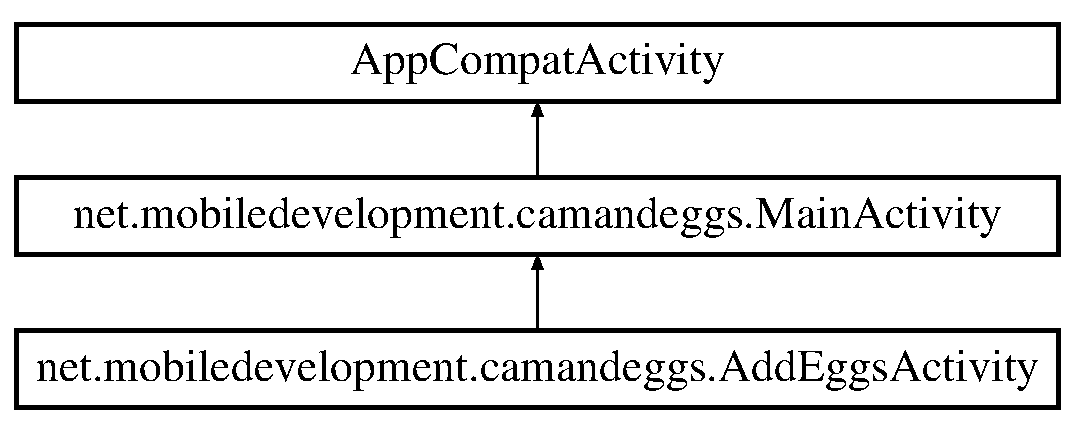
\includegraphics[height=3.000000cm]{classnet_1_1mobiledevelopment_1_1camandeggs_1_1_main_activity}
\end{center}
\end{figure}
\subsection*{Public Member Functions}
\begin{DoxyCompactItemize}
\item 
\mbox{\Hypertarget{classnet_1_1mobiledevelopment_1_1camandeggs_1_1_main_activity_ab3d2937015b4acf291bbc0c2703a6410}\label{classnet_1_1mobiledevelopment_1_1camandeggs_1_1_main_activity_ab3d2937015b4acf291bbc0c2703a6410}} 
void {\bfseries web\+Cam\+Load} (Web\+View wv, String url)
\item 
boolean \hyperlink{classnet_1_1mobiledevelopment_1_1camandeggs_1_1_main_activity_ab170f26993d4cca2a6932e5d7e780155}{on\+Create\+Options\+Menu} (Menu menu)
\item 
\mbox{\Hypertarget{classnet_1_1mobiledevelopment_1_1camandeggs_1_1_main_activity_ac718827b27f95f142684757a8087f2de}\label{classnet_1_1mobiledevelopment_1_1camandeggs_1_1_main_activity_ac718827b27f95f142684757a8087f2de}} 
boolean {\bfseries on\+Options\+Item\+Selected} (Menu\+Item item)
\end{DoxyCompactItemize}
\subsection*{Public Attributes}
\begin{DoxyCompactItemize}
\item 
\mbox{\Hypertarget{classnet_1_1mobiledevelopment_1_1camandeggs_1_1_main_activity_a97160c3eb4058966248714309ec8a36a}\label{classnet_1_1mobiledevelopment_1_1camandeggs_1_1_main_activity_a97160c3eb4058966248714309ec8a36a}} 
Web\+View {\bfseries web\+View\+Cam}
\item 
\mbox{\Hypertarget{classnet_1_1mobiledevelopment_1_1camandeggs_1_1_main_activity_adb85cb0ddaf038354e363e57a4738011}\label{classnet_1_1mobiledevelopment_1_1camandeggs_1_1_main_activity_adb85cb0ddaf038354e363e57a4738011}} 
String {\bfseries url\+String}
\end{DoxyCompactItemize}
\subsection*{Protected Member Functions}
\begin{DoxyCompactItemize}
\item 
void \hyperlink{classnet_1_1mobiledevelopment_1_1camandeggs_1_1_main_activity_a7e78ddf7c51cf7932de66127ed304ef0}{on\+Create} (Bundle saved\+Instance\+State)
\end{DoxyCompactItemize}


\subsection{Member Function Documentation}
\mbox{\Hypertarget{classnet_1_1mobiledevelopment_1_1camandeggs_1_1_main_activity_a7e78ddf7c51cf7932de66127ed304ef0}\label{classnet_1_1mobiledevelopment_1_1camandeggs_1_1_main_activity_a7e78ddf7c51cf7932de66127ed304ef0}} 
\index{net\+::mobiledevelopment\+::camandeggs\+::\+Main\+Activity@{net\+::mobiledevelopment\+::camandeggs\+::\+Main\+Activity}!on\+Create@{on\+Create}}
\index{on\+Create@{on\+Create}!net\+::mobiledevelopment\+::camandeggs\+::\+Main\+Activity@{net\+::mobiledevelopment\+::camandeggs\+::\+Main\+Activity}}
\subsubsection{\texorpdfstring{on\+Create()}{onCreate()}}
{\footnotesize\ttfamily void net.\+mobiledevelopment.\+camandeggs.\+Main\+Activity.\+on\+Create (\begin{DoxyParamCaption}\item[{Bundle}]{saved\+Instance\+State }\end{DoxyParamCaption})\hspace{0.3cm}{\ttfamily [protected]}}

for (int i = 0; i $<$= server\+List.\+size(); i++)\{ if (spinner.\+get\+Selected\+Item().to\+String() == server\+List.\+get(i).get\+I\+P()) \{ db.\+delete\+Server(server\+List.\+get(i)); break; \} else\{ Message.\+message(get\+Application\+Context(), \char`\"{}\+Could not remove address.\char`\"{}); \} \}\mbox{\Hypertarget{classnet_1_1mobiledevelopment_1_1camandeggs_1_1_main_activity_ab170f26993d4cca2a6932e5d7e780155}\label{classnet_1_1mobiledevelopment_1_1camandeggs_1_1_main_activity_ab170f26993d4cca2a6932e5d7e780155}} 
\index{net\+::mobiledevelopment\+::camandeggs\+::\+Main\+Activity@{net\+::mobiledevelopment\+::camandeggs\+::\+Main\+Activity}!on\+Create\+Options\+Menu@{on\+Create\+Options\+Menu}}
\index{on\+Create\+Options\+Menu@{on\+Create\+Options\+Menu}!net\+::mobiledevelopment\+::camandeggs\+::\+Main\+Activity@{net\+::mobiledevelopment\+::camandeggs\+::\+Main\+Activity}}
\subsubsection{\texorpdfstring{on\+Create\+Options\+Menu()}{onCreateOptionsMenu()}}
{\footnotesize\ttfamily boolean net.\+mobiledevelopment.\+camandeggs.\+Main\+Activity.\+on\+Create\+Options\+Menu (\begin{DoxyParamCaption}\item[{Menu}]{menu }\end{DoxyParamCaption})}

Tool bar options menu 

The documentation for this class was generated from the following file\+:\begin{DoxyCompactItemize}
\item 
Google Drive/\+C\+C\+B\+C/\+C\+S\+I\+T166/\+Camand\+Eggs/app/src/main/java/net/mobiledevelopment/camandeggs/Main\+Activity.\+java\end{DoxyCompactItemize}

\hypertarget{classnet_1_1mobiledevelopment_1_1camandeggs_1_1_message}{}\section{net.\+mobiledevelopment.\+camandeggs.\+Message Class Reference}
\label{classnet_1_1mobiledevelopment_1_1camandeggs_1_1_message}\index{net.\+mobiledevelopment.\+camandeggs.\+Message@{net.\+mobiledevelopment.\+camandeggs.\+Message}}
\subsection*{Static Public Member Functions}
\begin{DoxyCompactItemize}
\item 
\mbox{\Hypertarget{classnet_1_1mobiledevelopment_1_1camandeggs_1_1_message_a4747588bc5300eda5350425cf9114151}\label{classnet_1_1mobiledevelopment_1_1camandeggs_1_1_message_a4747588bc5300eda5350425cf9114151}} 
static void {\bfseries message} (Context context, String message)
\end{DoxyCompactItemize}


The documentation for this class was generated from the following file\+:\begin{DoxyCompactItemize}
\item 
/\+Users/robbwise/\+Google Drive/\+C\+C\+B\+C/\+C\+S\+I\+T166/\+Camand\+Eggs/app/src/main/java/net/mobiledevelopment/camandeggs/Message.\+java\end{DoxyCompactItemize}

\hypertarget{classnet_1_1mobiledevelopment_1_1camandeggs_1_1_server}{}\section{net.\+mobiledevelopment.\+camandeggs.\+Server Class Reference}
\label{classnet_1_1mobiledevelopment_1_1camandeggs_1_1_server}\index{net.\+mobiledevelopment.\+camandeggs.\+Server@{net.\+mobiledevelopment.\+camandeggs.\+Server}}
\subsection*{Public Member Functions}
\begin{DoxyCompactItemize}
\item 
\mbox{\Hypertarget{classnet_1_1mobiledevelopment_1_1camandeggs_1_1_server_a773bd30a67a11c01639d96bf5205a762}\label{classnet_1_1mobiledevelopment_1_1camandeggs_1_1_server_a773bd30a67a11c01639d96bf5205a762}} 
{\bfseries Server} (String ip)
\item 
\mbox{\Hypertarget{classnet_1_1mobiledevelopment_1_1camandeggs_1_1_server_a2c9a1872e2e6ff97b8f4ac9cb34d71f5}\label{classnet_1_1mobiledevelopment_1_1camandeggs_1_1_server_a2c9a1872e2e6ff97b8f4ac9cb34d71f5}} 
int {\bfseries get\+Id} ()
\item 
\mbox{\Hypertarget{classnet_1_1mobiledevelopment_1_1camandeggs_1_1_server_ac4fc0647dde28db00e875573530b860c}\label{classnet_1_1mobiledevelopment_1_1camandeggs_1_1_server_ac4fc0647dde28db00e875573530b860c}} 
String {\bfseries get\+IP} ()
\item 
\mbox{\Hypertarget{classnet_1_1mobiledevelopment_1_1camandeggs_1_1_server_a1be30996fde32971d7414df0adf7df1b}\label{classnet_1_1mobiledevelopment_1_1camandeggs_1_1_server_a1be30996fde32971d7414df0adf7df1b}} 
void {\bfseries set\+Id} (int i)
\item 
\mbox{\Hypertarget{classnet_1_1mobiledevelopment_1_1camandeggs_1_1_server_a54a629226e0ed116a93405107d91b8b3}\label{classnet_1_1mobiledevelopment_1_1camandeggs_1_1_server_a54a629226e0ed116a93405107d91b8b3}} 
void {\bfseries set\+IP} (String i)
\item 
\mbox{\Hypertarget{classnet_1_1mobiledevelopment_1_1camandeggs_1_1_server_aa2e205a94f8c7ae112cc50c308cd0000}\label{classnet_1_1mobiledevelopment_1_1camandeggs_1_1_server_aa2e205a94f8c7ae112cc50c308cd0000}} 
String {\bfseries to\+String} ()
\end{DoxyCompactItemize}


\subsection{Detailed Description}
Created by robbwise on 3/28/18. 

The documentation for this class was generated from the following file\+:\begin{DoxyCompactItemize}
\item 
/\+Users/robbwise/\+Google Drive/\+C\+C\+B\+C/\+C\+S\+I\+T166/\+Camand\+Eggs/app/src/main/java/net/mobiledevelopment/camandeggs/Server.\+java\end{DoxyCompactItemize}

%--- End generated contents ---

% Index
\backmatter
\newpage
\phantomsection
\clearemptydoublepage
\addcontentsline{toc}{chapter}{Index}
\printindex

\end{document}
